\documentclass[a4paper,12pt]{article}

\usepackage{amsmath,amssymb,multicol,tikz}
\usepackage[margin=2cm]{geometry}
%\usetikzlibrary{calc}
\usepackage{amsmath}
\usepackage{amsthm}
\usepackage{thmtools}
\usepackage{hyperref}
\usepackage{enumerate}
\usepackage{xcolor}
\usepackage{fancyvrb}

\pagestyle{empty}

\newcommand\Q{\mathbf{Q}}
\newcommand\R{\mathbf{R}}
\newcommand\Z{\mathbf{Z}}

\usepackage{array}
\newcolumntype{P}[1]{>{\centering\arraybackslash}p{#1}}

\newcommand\indd{${}$\hspace{20pt}}

\declaretheoremstyle[headfont=\normalfont\bfseries,notefont=\mdseries\bfseries,bodyfont = \normalfont,headpunct={:}]{normalhead}
\declaretheorem[name={Uzdevums}, style=normalhead,numberwithin=section]{problem}

\setcounter{section}{117}

\setlength\parindent{0pt}

\begin{document}

\clearpage
\begin{center}
\parbox{3.5cm}{\flushleft\bf Gadījumlielumi \newline ATV} \hfill {\bf\LARGE Uzdevumi nedēļai \#17} \hfill \parbox{3.5cm}{\flushright\bf 2021-04-28} %\\[2pt]
\end{center}

%\hrule\vspace{2pt}\hrule
\hrule



\vspace{10pt}
\begin{problem}
Iedomāsimies, ka mums ir divi metamie kauliņi: viens ar $6$ skaldnēm (ar skaitļiem $1,\dots,6$) un otrs ar $8$ skaldnēm  
(ar skaitļiem $1,\dots,8$). Uz abiem reizē uzmet skaitļus. Ar $T$ apzīmējam gadījumlielumu \textendash{} uz abiem kauliņiem uzmesto 
skaitļu summu. 
\begin{figure}[!htb]
\center{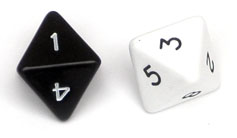
\includegraphics[width=1in]{atv-17/octahedron-dice.png}}
\caption{\label{fig:octahedron-dice} Oktaedra formas kauliņi ar $8$ skaldnēm.}
\end{figure}
\begin{enumerate}[(a)]
\item Katrai no iespējamajām $T$ vērtībām $a$ atrast, cik veidos to var uzmest (un kāda ir varbūtība, ka tieši šo 
vērtību uzmetīs: $p(T = a)$). 
\item Atrast $E(T)$ \textendash{} gadījumlieluma vidējo vērtību. 
\item Atrast $p(T = E(T))$ (t.i.\ varbūtību, ka $T$ būs vienāds pats ar savu vidējo vērtību).
\item Atrast varbūtības $p(T = (E(T)-1))$ un $p(T = (E(T)+1))$. 
\item Atrast dispersiju $V(T)$. To rēķina pēc formulas $V(T) = E((T - E(T))^2)$.
\end{enumerate}
\end{problem}


\vspace{10pt}
\begin{problem}
Vienā eksperimentā ripinām divus parastus metamos kauliņus (uz tiem var uzmest skaitļus $1,\ldots,6$ ar vienādām varbūtībām). 
Definējam šādus notikumus: 
\[ \left\{ \begin{array}{l}
A := \text{uz abiem kauliņiem uzmesto punktu summa ir $7$},\\
B := \text{uz pirmā kauliņa uzmeta $2$},\\
C := \text{uz otrā kauliņa uzmeta $5$}.\\
D := \text{uz abiem kauliņiem uzmesto punktu summa ir vismaz $7$},\\
\end{array} \right. \]
\begin{enumerate}[(a)]
\item Atrast nosacītās varbūtības $p(B|A)$ un $p(B|D)$?
\item Vai notikumi $A,B,C$ ir pa pāriem neatkarīgi? (Jāpārbauda trīs vienādības: $p(A \cap B) = p(A)p(B)$, $p(A \cap C) = p(A)p(C)$, $p(B \cap C) = p(B)p(C)$.)
\item Vai notikumi $B,C,D$ ir pa pāriem neatkarīgi? 
\item Vai notikumi $A,B,C$ ir savstarpēji neatkarīgi?\\
{\em Piezīme.} Trīs notikumi $A,B,C$ ir savstarpēji neatkarīgi, ja tie ir pa pāriem neatkarīgi un 
bez tam arī visu trīs notikumu šķēluma varbūtība $p(A \cap B \cap C) = p(A)p(B)p(C)$.
\end{enumerate}
\end{problem}


\vspace{10pt}
\begin{problem}
Teātrī iegāja $n$ cilvēki; katrs nodeva garderobē savu cepuri. Izejot no teātra garderobists cepures sajauca (visas $n!$ cepuru permutācijas
var notikt ar vienādu varbūtību). 
\begin{enumerate}[(a)]
\item Atrast varbūtību notikumam, ka tieši trīs cilvēki saņēma atpakaļ savas cepures tad, ja $n=4$, $n=5$, $n=6$. 
(Apzīmējam šīs varbūtības attiecīgi ar $p_4$, $p_5$, $p_6$.)
\item 
Pamatot, ka $p_n$ apmierina vienādību: 
\[ p_n = \frac{1}{3!} \left( \frac{1}{0!} - \frac{1}{1!} + \frac{1}{2!} - \frac{1}{3!} + \ldots + (-1)^{n-3} \frac{1}{(n-3)!} \right). \]
{\em Ieteikums.} Var izmantot ieslēgšanas-izslēgšanas principu (principle of inclusion-exclusion) par elementu skaitu kopu apvienojumā.
\end{enumerate}
\end{problem}




\vspace{10pt}
\begin{problem}
Divi spēlētāji spēlē sekojošu spēli ar vienu monētu (monēta ir simetriska un abi iznākumi notiek ar vienādām varbūtībām):
\begin{itemize}
\item Spēlētājs $A$ izvēlas virknīti no $3$ burtiem; katrs burts ir {\tt C} (cipars) vai {\tt Ģ} (ģerbonis).
\item Spēlētājs $B$ izvēlas citu virknīti no $3$ burtiem; arī katrs burts ir {\tt C} vai {\tt Ģ}.
\item Pēc tam viņi met monētu, kamēr katrs no viņiem ir ieraudzījis savu virknīti trīs pēc kārtas sekojošos metienos. 
\end{itemize}
Pieņemsim, ka spēlētājs $A$ izvēlējās {\tt "CCĢ"}, bet spēlētājs $B$ izvēlējās {\tt "ĢCC"}. 
Ar $X$ apzīmēsim gadījumlielumu ar vērtībām $n \in \{ 3,4,5,\ldots \}$, kas parāda, cik reizes bija jāmet monēta, lai metienu rezultātos
pirmo reizi parādītos spēlētāja $A$ virknīte {\tt "CCĢ"}.
\begin{enumerate}[(a)]
\item Atrast $p(X=n)$ pie $n=3,4,5,6$ (t.i. varbūtību, ka virknītes "CCĢ" iegūšanai monēta bija jāmet tieši $3$ reizes, tieši $4$ reizes, utt.). 
\item Atrast vidējo vērtību $E(X)$ (ja grūti precīzi summēt šo virkni, var izmantot arī Python programmu - piemēram, uz datora ``izspēlēt'' 
$1000$ monētu mešanas virknītes un atrast, cik ātri tur parādās virknīte {\tt "CCĢ"}. Sk. funkciju {\tt random.choices(...)} Attēlā~\ref{fig:python-choices}.
\begin{figure}[!htb]
\center{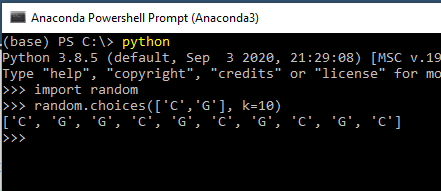
\includegraphics[width=3in]{atv-17/python-choices.png}}
\caption{\label{fig:python-choices} Nejaušas virknes ({\tt list}) iegūšana Python.}
\end{figure}
\item Atrast varbūtību, ka spēlētājs $A$ uzvar spēlētāju $B$ (t.i.\ viņa virknīte parādās ātrāk).
\item Kādu $3$-burtu virknīti ir visizdevīgāk izvēlēties, ja esat spēlētājs $A$ un varat izvēlēties pirmais?
\end{enumerate}
\end{problem}





\vspace{10pt}
\begin{problem}
$1000$ cilvēkus testē uz kādu slimību; tests dod pareizu atbildi ar 90\% varbūtību (ar 10\% varbūtību tas kļūdās vienā vai otrā virzienā \textendash{}
ir pozitīvs veseliem cilvēkiem vai arī negatīvs slimiem). Zināms, ka  40\% no visiem $1000$ cilvēkiem ir šī slimība.
\begin{enumerate}[(a)]
\item Kāda ir varbūtība, ka testa rezultāts konkrētam cilvēkam būs pozitīvs?
\item Kādam cilvēkam testa rezultāts ir pozitīvs. Kāda varbūtība, ka viņam tiešām ir šī slimība?
\end{enumerate}
\end{problem}

\end{document}

